\documentclass{article}
\usepackage{url}
\usepackage{amsmath}
\usepackage{amsfonts}
\usepackage{amssymb}
\usepackage{graphicx}
\usepackage{arxiv_new}
\usepackage{nicefrac}
\usepackage{microtype}
\usepackage{hyperref}
\usepackage{mathtools}
\usepackage{subcaption}
\usepackage{booktabs}
\usepackage{xcolor}

% ---- Author-year citations rendered as (Author Year) with round parens ----
% Uses the article class's \bibitem[label]{key} mechanism so \cite prints the
% given label.  Swap default square brackets for round parens (both for in-text
% \cite and for the bibliography list marker).
\makeatletter
\renewcommand{\@cite}[2]{(#1\if@tempswa , #2\fi)}
\renewcommand{\@biblabel}[1]{}
\makeatother

% ============================================================================
% Rule-table structure of life-like cellular automata. Self-contained; inline
% bibliography. AGENT: reconcile figure filenames in \includegraphics at compile.
% ============================================================================

\begin{document}

\title{Rule-table structure of life-like cellular automata:\\
activity, asymmetry, sensitivity,\\
and the propagation--storage factorisation}
\author{Yair Cohen}
\date{\today}
\maketitle

\begin{abstract}
What structure on the rule space of a cellular-automaton family exposes which
rules can support which behaviours? For life-like rules---the two-dimensional
family that contains Conway's Game of Life---the standard coordinate is Langton's
$\lambda$, a single number measuring how much of the rule table fires, long known
to be too coarse. We argue for a small, symmetry-organised set
of rule-table coordinates and, more pointedly, for what such coordinates can and
cannot do: built from cardinalities, they are \emph{necessary but not sufficient}
to certify a rule's behaviour, yet they can \emph{exclude} behaviour outright. We
split Langton's parameter into its birth and survival contributions, whose
difference is a birth--survival asymmetry that separates birth-dominated from
survival-dominated rules---a coordinate specific to the outer-totalistic
family (whose rule table factors by cell state into a birth set and a
survival set), not a re-parameterisation of $\lambda$ that carries over to
general CA. We add the average Boolean-derivative sensitivity of
Vichniac and Binder, extended to the life-like family in closed form, whose
centre-cell component vanishes exactly on the fully totalistic rules (those whose
birth and survival conditions coincide). Combined with an exhaustive enumeration,
across all $262{,}144$ rules, of the compact gliders, still lifes and oscillators
each rule supports, these coordinates expose a clean structure. Propagation and
storage separate along the asymmetry axis: the birth rule is a narrow gate
deciding whether anything can move, the survival rule tunes how much structure
persists once that gate is open, and---at the compact footprint---the rules
supporting gliders are systematically birth-light and survival-rich. One exclusion
is exact: no fully totalistic ($B=S$) rule supports a compact ($3{\times}3$,
period $\le16$) glider, an exhaustively verified combinatorial exclusion that the
vanishing centre-cell sensitivity explains, while the same rules oscillate at
near-background rate---localising it to translation rather than to in-place
recurrence. Two dynamical results frame the whole: rules that support a glider yet
rarely or never produce one under random sampling show that capability is
\emph{certifiable} from the table but its expression only \emph{estimable} from
dynamics; and, conversely, of the uncatalogued rules whose dynamics we screen for
a Game-of-Life--like object ecology, those matching it richly are all Conway or
HighLife variants differing only on neighbour counts their trajectories never
visit---so table difference need not mean behavioural difference. The coordinates
organise the family not by certifying capability but by carving the regions where
it is possible---and, on the fully totalistic submanifold, the region where it is
impossible.
\end{abstract}

\section{Introduction}

A cellular automaton (CA) updates a lattice of cells in parallel by a rule that
depends only on each cell and a small neighbourhood, yet even tiny rule families
produce propagating structures, long transients and universal
computation~\cite{vonneumann1966,wolfram1983,berlekamp1982}. This paper concerns
a basic organisational question for one such family: given the $262{,}144$
two-dimensional outer-totalistic ``life-like'' rules, what coordinates on the
rule table expose the structure of behavioural capability---which regions support
propagation, which support storage, and which exclude a behaviour outright? A
life-like rule
is fixed by two subsets $B,S\subseteq\{0,\dots,8\}$: a dead cell is born if its
live-neighbour count lies in $B$, and a live cell survives if its count lies in
$S$. The family contains Conway's Game of Life and its named variants---HighLife,
Day~\&~Night, Seeds, $2{\times}2$, Replicator,
Maze~\cite{gardner1970,adamatzky2010,eppstein2010}.

The standard coordinate is Langton's $\lambda$, the fraction of the rule table
that yields a live successor~\cite{langton1990}. Sweeping $\lambda$ moves through
frozen, periodic, complex and chaotic regimes, and the intermediate ``edge of
chaos'' was conjectured to host maximal computational capability. But $\lambda$
is a single number summarising an $18$-bit table: two rules that differ in
\emph{which} neighbour counts fire, not just \emph{how many}, collapse onto the
same point, and evolved-CA studies found no sharp critical
$\lambda$~\cite{mitchell1993}.

\paragraph{Necessary, not sufficient.}
This collapse is not a defect to be engineered away but a structural fact worth
stating plainly, because it sets the ceiling on what any cardinality-based
coordinate can do. Both $\lambda$ and the asymmetry $\delta$ we introduce below
are functions of the cardinalities $(|B|,|S|)$ alone; there are only $10\times10$
such pairs, so the entire $(\lambda,\delta)$ plane has at most $100$ occupied
points, each shared by thousands of behaviourally distinct rules. A coordinate
this coarse can never \emph{certify} that a rule does something---any value it
takes is shared by a crowd. What it can do is the opposite: place a rule in a
region, and---in the limiting case---\emph{exclude} a behaviour entirely. Our
results are organised around this asymmetry. The asymmetry coordinate $\delta$
locates where capability concentrates (a necessary condition); the centre-bit
sensitivity $\mu_{\text{centre}}$ supplies the one exact exclusion, ruling out
compact gliders on the fully totalistic submanifold outright.

\paragraph{The coordinates.}
We add two complementary rule-table coordinates. The first comes from splitting
$\lambda$ into its birth and survival halves, $\lambda_B=|B|/9$ and
$\lambda_S=|S|/9$; their difference $\delta=\lambda_B-\lambda_S=(|B|-|S|)/9$ is a
birth--survival asymmetry, the antisymmetric companion to Langton's $\lambda$,
and the coordinate on which our central structural result is read. The split
is only defined for outer-totalistic families whose rule table separates by
cell state (dead-cell births $B$ vs.\ live-cell survivals $S$); in that sense
$\delta$ is a coordinate for this family, not a re-parameterisation of
$\lambda$ that generalises to CA whose transitions do not factor this way.
The second is
the average Boolean-derivative \emph{sensitivity} $\mu$---the probability that
flipping one input bit of the neighbourhood flips the output---introduced for CA
by Vichniac~\cite{vichniac1990} and used as an a-priori ordering parameter by
Binder~\cite{binder1993}. For life-like rules $\mu$ admits a closed form that
splits into a centre-bit part $\mu_{\text{centre}}$ and a neighbour part
$\mu_{\text{neigh}}$, and the centre part vanishes exactly on the diagonal $B=S$.
The two new coordinates are independent, not interchangeable: under the
birth/survival swap $\tau\!:\!(B,S)\!\mapsto\!(S,B)$, $\delta$ is odd while $\mu$
is even, so $\mu$ cannot tell a rule from its $B\leftrightarrow S$ mirror and
$\delta$ can. With $\lambda$ and the bit-flip complement $\sigma$ they organise
the rule table into a four-sector parity decomposition, closed by one further
coordinate $\delta_{\text{edge}}$ (\S\ref{sec:symm}).

\paragraph{Findings.}
Pairing this coordinate system with an exhaustive combinatorial enumeration of
every rule's compact-spaceship, still-life and oscillator support, we establish
three results. (i)~A hierarchical factorisation of capacity, read off the
birth--survival asymmetry $\delta$: the birth set is a narrow gate that decides
whether anything can propagate, while the survival set tunes how much structure
is stored within that gate. The gate structure is robust across seed footprints
(the $3{\times}3$ propagation-enabling birth sets are a subset of the
$4{\times}4$ ones, both dominated by small birth sets); at the compact footprint
this shows up as a clean fingerprint---the rules supporting compact gliders are
systematically birth-light and survival-rich ($\delta<0$)---which is the paper's
central structural finding, and which we show is specific to the compact footprint
and dilutes as the window widens. (ii)~Three coordinate projections of the rule
table---the Binder $(\lambda,\mu)$ plane and its $(\delta,\mu)$ and
$(\lambda,\delta)$ companions---that organise the family non-trivially, in which
the $512$ fully totalistic rules occupy a sharply identifiable locus. (iii)~A
total exclusion of $B=S$ rules from compact ($3{\times}3$, period $\le16$)
gliders---certified by the exhaustive enumeration and explained by the vanishing
centre-cell sensitivity $\mu_{\text{centre}}=0$---which the oscillator enumeration
localises to translation rather than to in-place recurrence, and which softens
into a widening handicap rather than vanishing at larger footprints. Two
dynamical results frame these. First, a population of rules that support a glider
combinatorially yet rarely or never express one under random sampling shows that
capability is a rule-table property, distinct from what random dynamics reveal
(auxiliary dynamical observables are correspondingly reframed as regime
descriptors, not capability detectors). Second, and conversely, a table-blind
screen of the uncatalogued build-and-hold rules for Game-of-Life--like dynamics
returns a richly Life-like ecology only for Conway and HighLife variants---rules
whose tables differ from an anchor's solely on neighbour counts their trajectories
never visit---so that table difference need not imply behavioural difference. The
exact bit-flip
duality $\sigma$ (\S\ref{sec:symm}) is used only to gauge-fix that auxiliary
dynamical sweep (Appendix~\ref{app:dynamical}).

\section{Methods}

\subsection{Notation and computed quantities}
\label{sec:notation}

Table~\ref{tab:notation} collects every rule-table and dynamical quantity used in
the paper. The rule-table coordinates are defined in
\S\ref{sec:coords}--\S\ref{sec:symm}, the combinatorial indices in
\S\ref{sec:enum}, and the single dynamical probe in \S\ref{sec:dyn}. All
rule-table quantities are functions of $(B,S)$ alone and are independent of any
simulation protocol.

\begin{table}[h]
\centering
\small
\renewcommand{\arraystretch}{1.25}
\begin{tabular}{llp{6.2cm}}
\toprule
Symbol & Definition & Measures \\
\midrule
$\lambda_B,\lambda_S$ & $|B|/9,\ |S|/9$ & how much of the birth / survival rule fires, as a fraction \\
$\lambda$ & $\tfrac12(\lambda_B+\lambda_S)=(|B|+|S|)/18$ & Langton's parameter: the overall fraction of the table that fires \\
$\delta$ & $\lambda_B-\lambda_S=(|B|-|S|)/9$ & birth-versus-survival imbalance: positive if the rule births more than it preserves, negative if it preserves more than it births; the paper's factorisation axis \\
$\mu$ & avg.\ over inputs/bit-positions of $P[\text{flip flips output}]$ & sensitivity: how often flipping one input cell flips the rule's output \\
$\mu_{\text{centre}}$ & $P[n\in B\triangle S],\ n\sim\mathrm{Bin}(8,\tfrac12)$ & how much a cell's \emph{own} state matters to its fate; zero exactly when $B=S$ \\
$\mu_{\text{neigh}}$ & binomially-weighted edge density of $B,S$ & how ``jagged'' the thresholds are---how often firing switches on/off between adjacent neighbour counts \\
$e(M)$ & $\#\{k:\mathbf 1[k\in M]\neq\mathbf 1[k{+}1\in M]\}$ & number of on/off switches in a set $M$ as the count rises \\
$\delta_{\text{edge}}$ & $(e(B)-e(S))/8$ & whether the birth threshold is more or less contiguous than the survival one \\
$\Sigma$ & \# distinct $3{\times}3$ $D_4$-orbit spaceships, $T\le16$ & how many compact gliders the rule can support at all \\
$\#\mathrm{SL}$ & \# distinct $3{\times}3$ $D_4$-orbit still lifes ($T{=}1$) & how many small static patterns the rule can hold fixed \\
$\Omega$ & \# distinct $3{\times}3$ $D_4$-orbit oscillators, $2\le T\le16$ & how many small patterns the rule can hold as in-place blinkers \\
$\mathcal{B}_{\text{prop}},\mathcal{B}_{\text{osc}},\mathcal{B}_{\text{sl}}$ & birth sets with $\ge4$ companion $S$ giving $\Sigma>0$ ($\Omega>0$; $\#\mathrm{SL}>0$) & which birth rules ``open the gate'' for propagation / oscillation / storage \\
$\mathcal{G}^{*}_{\text{alt}}$ & peak off-axis residual spatiotemporal autocorrelation & whether random dynamics actually show a coherent moving structure \\
$\mathrm{gap}$ & $\mu-\langle\mathrm{sens}\rangle_{\text{traj}}$ & how much the dynamics under-use the rule's intrinsic sensitivity \\
\bottomrule
\end{tabular}
\caption{Notation and computed quantities. The first eight rows are rule-table
coordinates (functions of $(B,S)$ alone); $\Sigma$, $\#\mathrm{SL}$, $\Omega$ count
the small moving / static / blinking patterns a rule supports; the last two are
the single dynamical probe. $B\triangle S=(B\setminus S)\cup(S\setminus B)$ is the
set of counts where birth and survival disagree; $\tau$ and $\sigma$ are the swap
and complement symmetries of \S\ref{sec:symm}; $D_4$ is the eight-fold symmetry
group of the square.}
\label{tab:notation}
\end{table}

\subsection{Rule-space coordinates: $\lambda$, $\delta$}
\label{sec:coords}

Each rule splits its look-up table into a birth component $B$ on dead cells and a
survival component $S$ on live cells, so we define $\lambda_B=\tfrac19\sum_k\mathbf
1[k\in B]$, $\lambda_S=\tfrac19\sum_k\mathbf 1[k\in S]$, the Langton parameter
$\lambda=\tfrac12(\lambda_B+\lambda_S)$, and its antisymmetric companion
\begin{equation}
  \delta=\lambda_B-\lambda_S=\frac{|B|-|S|}{9}.
\end{equation}
The pair $(\lambda,\delta)$ is a bijective reparameterisation of
$(\lambda_B,\lambda_S)$.

\paragraph{$\delta=0$ versus $B=S$.}
These loci are easily conflated but combinatorially distinct, and the distinction
is exactly the necessary/sufficient one. $\delta=0$ is the equal-cardinality
submanifold $|B|=|S|$, containing $\sum_k\binom{9}{k}^2=\binom{18}{9}=48{,}620$
rules; the strictly diagonal $B=S$ (the fully totalistic rules) is far smaller,
only $512$. This $B=S$ set is not new: it is the classical \emph{totalistic}
Life-like subclass, whose members are those for which birth and survival coincide
(up to the usual centre-counting convention); what is new is its characterisation
as the exact zero set of the centre-cell sensitivity below, and the compact-glider
exclusion we prove on it. Equivalently, writing the unweighted set distance $|B\triangle S|$
(the number of counts in exactly one of $B,S$), $B=S$ is $|B\triangle S|=0$ while
$\delta=0$ is only $|B|=|S|$, so $\{B=S\}\subsetneq\{\delta=0\}$. The coordinate
that isolates $B=S$ exactly is the centre-bit sensitivity introduced next, of
which $|B\triangle S|$ is the unweighted shadow: we show in \S\ref{sec:results-mu}
that $B=S$ is precisely the $\mu_{\text{centre}}=0$ locus.

\subsection{Sensitivity coordinate $\mu$ (Boolean derivative)}
\label{sec:mu}

The $(\lambda,\delta)$ coordinates summarise activity but say nothing about how
strongly a rule responds to single-bit perturbations of its input. The standard
summary is the average Boolean derivative~\cite{vichniac1990,binder1993}: for a
rule with $N$ input bits and binary output $o$,
\begin{equation}
  \mu=\frac{1}{N\,2^{N}}\sum_{x\in\{0,1\}^N}\sum_{i=1}^{N}
  \bigl[o(x\oplus e_i)\neq o(x)\bigr],
\end{equation}
the probability that a single-bit flip flips the output; it is closely related to
Wuensche's $Z$ parameter~\cite{wuensche1999}. For an outer-totalistic life-like
rule on the Moore neighbourhood the $N=9$ inputs split as one centre bit and $8$
neighbour bits, and the table depends on inputs only through $(c,n)$ with $c$ the
centre value and $n$ the neighbour count. With $o(c,n)=\mathbf 1[c{=}0]\,\mathbf
1[n\in B]+\mathbf 1[c{=}1]\,\mathbf 1[n\in S]$, the centre and neighbour
contributions have closed forms
\begin{align}
  \mu_{\text{centre}}&=\frac{1}{2^{8}}\sum_{n=0}^{8}\binom{8}{n}\,
    \mathbf 1[n\in B\triangle S],\\
  \mu_{\text{neigh}}&=\frac{1}{2^{8}}\sum_{k=0}^{7}\binom{7}{k}
    \bigl(\mathbf 1[k\in B\triangle(B{-}1)]+\mathbf 1[k\in S\triangle(S{-}1)]\bigr),
\end{align}
with $\mu=\tfrac19(\mu_{\text{centre}}+8\,\mu_{\text{neigh}})$. The notation needs a
word. $B\triangle S$ is the \emph{symmetric difference} of the two sets: the
neighbour counts at which birth and survival \emph{disagree}---a count belongs to
$B\triangle S$ when it triggers exactly one of the two, birth or survival, but not
both and not neither. For Conway ($B=\{3\}$, $S=\{2,3\}$) the two sets share the
count $3$ and differ only at $2$, so $B\triangle S=\{2\}$: a cell's own state
matters only when it has exactly two live neighbours. The companion term
$B\triangle(B{-}1)$ applies the same ``disagree'' operation to a set and its
shift-by-one, which simply marks the \emph{edges} of $B$---the counts where
membership switches on or off as the neighbour total climbs by one (the symbol
$\oplus$ is this exclusive-or of the two adjacent memberships). Three consequences
follow.
\begin{enumerate}
  \item \textbf{$\mu_{\text{centre}}=0$ is the $B=S$ submanifold.} By the formula
    $\mu_{\text{centre}}=0$ iff $B\triangle S=\varnothing$, i.e.\ $B=S$. So
    $\mu_{\text{centre}}$ is exactly the binomially-weighted set distance from
    totalistic, and the $512$ fully totalistic rules are characterised a priori:
    they cannot respond differently to the centre cell's own state at any count.
  \item \textbf{$\mu_{\text{neigh}}$ counts birth/survival edges}; alternating
    sets such as $\{1,3,5,7\}$ (Replicator) maximise it.
  \item \textbf{$\mu$ is independent of $\lambda$}: one measures the fraction of
    table entries that fire, the other the fraction of input-bit flips that
    change the output. Together they form a Binder $(\lambda,\mu)$ plane
    (\S\ref{sec:results-mu}).
\end{enumerate}

\subsection{A symmetry-organised coordinate system}
\label{sec:symm}

The rule table carries two natural involutions,
\begin{equation}
  \tau:(B,S)\mapsto(S,B),\qquad
  \sigma:(B,S)\mapsto\bigl(\overline{\mathrm{rev}(S)},\overline{\mathrm{rev}(B)}\bigr),
\end{equation}
where $\mathrm{rev}(M)=\{8-k:k\in M\}$ and the bar is the complement in
$\{0,\dots,8\}$. $\tau$ swaps birth and survival; $\sigma$ is the bit-flip
duality, in the sense that if $g=\sigma(f)$ then $g(\lnot x)=\lnot f(x)$ for every
configuration. Both square to the identity, and the rule space falls into the
four parity sectors of $(\tau,\sigma)$. The Boolean-derivative formalism supplies
one further coordinate that completes the decomposition, the edge imbalance
$\delta_{\text{edge}}=(e(B)-e(S))/8$.

\paragraph{Parity table.}
We verified the action of $\tau$ and $\sigma$ on every coordinate by direct
evaluation on all $262{,}144$ rules (max residue $1.1\times10^{-16}$): $\lambda$
is ($\tau$-even, $\sigma$-odd; $\lambda\mapsto1-\lambda$); $\delta$ is
($\tau$-odd, $\sigma$-even; $\delta$ invariant under $\sigma$);
$\mu_{\text{centre}},\mu_{\text{neigh}},\mu$ are ($\tau$-even, $\sigma$-even); and
$\delta_{\text{edge}}$ is ($\tau$-odd, $\sigma$-odd). The load-bearing
observation is that $\lambda$ and $\mu$ are both $\tau$-even, so neither can
distinguish a rule from its $B\leftrightarrow S$ mirror; $\delta$ is the unique
$\tau$-odd coordinate among the activity/sensitivity axes, and is therefore the
natural birth-versus-survival scalar. Since $\sigma$ acts as
$(\lambda,\delta,\mu)\mapsto(1-\lambda,\delta,\mu)$, self-dual rules need not have
$\delta=0$---consistent with Day~\&~Night ($\delta=-\tfrac19$) being self-dual.
Pearson correlations across the full rule space are exactly zero between every
pair of $\{\lambda,\delta,\mu,\delta_{\text{edge}}\}$, as required by the
orthogonality of parity sectors under the uniform measure.

\paragraph{Roles of the coordinates.}
Each answers a distinct question the others structurally cannot, and the
necessary/sufficient distinction runs through all four. $\lambda$ places a rule on
the frozen$\to$chaotic spectrum but collapses rules of equal total firing
fraction, so it is a necessary entry point, never sufficient. $\delta$ is the
swap-odd factorisation axis: $\Sigma>0$ rules are birth-light and survival-rich
($\delta\approx-0.22$), the rule-table fingerprint of the $B$-gate / $S$-knob
structure (\S\ref{sec:results-factor}); without $\delta$ the claim cannot even be
stated. $\mu_{\text{centre}}$ is the one coordinate that excludes rather than
merely locates: $\mu_{\text{centre}}=0$ iff $B=S$, turning the empirical $B=S$
exclusion into a one-line characterisation (\S\ref{sec:results-sigma}).
$\mu_{\text{neigh}}$ measures threshold jaggedness but is swap-even and carries no
birth-versus-survival information; $\delta_{\text{edge}}$ is its swap-odd
companion, a secondary, mechanism-consistent preference for contiguous birth
thresholds (\S\ref{sec:results-factor}).

\subsection{Combinatorial enumeration: $\Sigma$, $\#\mathrm{SL}$, $\Omega$}
\label{sec:enum}

The following are functions of the rule table alone and independent of any
simulation protocol. For each rule we enumerate every $3{\times}3$ binary pattern
(reduced to its $D_4$ orbit representative) on a quiescent zero-padded background,
evolve it to $T_{\max}=16$, and classify the orbit by its return behaviour: a
nonzero-offset translated return is a \emph{spaceship} ($\Sigma$ counts distinct
orbit-representative spaceships, with period and velocity set); a same-position
return at period $2\le T\le16$ is an \emph{oscillator} ($\Omega$); a fixed pattern
($T{=}1$) is a \emph{still life} ($\#\mathrm{SL}$). $\Sigma$ asks ``can the rule
support a compact glider at all,'' independent of whether a random trajectory ever
exhibits one. A cheap pre-screen exploits that translated and stationary copies
both preserve the seed's live-cell count exactly: monitoring the running sum
rejects the great majority of rules within a few steps, leaving the small
fraction that warrant the full check.

\subsection{Dynamical probe and coherent-propagation index $\mathcal{G}^{*}$}
\label{sec:dyn}

To identify rules whose combinatorial propagation is or is not expressed by random
dynamics we run a single fixed sweep. For each rule we draw $5$ shared Bernoulli
ICs at density $\rho_0=0.30$ on a $128\times128$ torus, together with their
bit-flipped partners at density $0.70$ (the symmetric-IC ensemble; see
Appendix~\ref{app:dynamical}), evolve $600$ steps, and measure on the $200$-frame
tail a residual spatiotemporal autocorrelation $\mathcal{G}^{*}_{\text{alt}}$: a
coherent structure of period $T$ and velocity $(v_x,v_y)$ produces an off-axis
peak at $(\Delta t,\Delta x,\Delta y)=(T,-Tv_x,-Tv_y)$, validated by an injection
test in which an isolated Conway glider peaks at $(\Delta t{=}4,\Delta
x{=}{-}1,\Delta y{=}{-}1)$. We use $\mathcal{G}^{*}_{\text{alt}}$ only to flag
rules with no measurable coherent propagation; the remaining dynamical observables
are regime descriptors, deferred to Appendix~\ref{app:dynamical}.

\section{Results}

\subsection{The rule-table phase diagrams $(\lambda,\mu)$, $(\delta,\mu)$, $(\lambda,\delta)$}
\label{sec:results-mu}

The sensitivity coordinate places every rule on a second axis complementing
$\lambda$ (Figure~\ref{fig:planes}). The cloud of all $262{,}144$ rules forms a
structured band, and the $B=S$ submanifold ($\mu_{\text{centre}}=0$) traces a
sharply identifiable locus on which all $512$ fully totalistic rules lie.
Replicator sits at the top with $\mu=0.889$---centre-insensitive but maximally
neighbour-sensitive---showing $B=S$ is not synonymous with low sensitivity, only
with centre-flip insensitivity. The $424$ rules with $\Sigma>0$ cluster off that
locus at moderate $\lambda$ and $\mu\in[0.25,0.60]$; Conway ($\mu=0.35$) and
HighLife ($0.46$) are $\Sigma>0$ and lie in the cluster, while the storage-heavy
Class~IV anchor Day~\&~Night lies at the same moderate $\mu$ ($0.565$) yet is
itself $\Sigma=0$ (Figure~\ref{fig:joint})---a first
illustration that the moderate-$(\lambda,\mu)$ region is necessary for compact
propagation but does not certify it~\cite{wolfram1984}. ($2{\times}2$, another
Class~IV anchor with $\Sigma=0$, sits just above the band at $\mu=0.639$; both
rules are complex through engineered rather than compact-glider dynamics, a point
we return to in \S\ref{sec:disc-conway}.) The middle panel shows the
same rules in $(\delta,\mu)$, where the $\Sigma>0$ cluster sits at
$\delta\approx-0.2$ (the birth-light/survival-rich offset of
\S\ref{sec:results-factor}) and the $B=S$ rules collapse to the line $\delta=0$;
the right panel shows the $(\lambda,\delta)$ projection, where the $\Sigma>0$
rules form a diamond near $(0.4,-0.2)$. We do not claim the planes as a sharp
classifier: the $\Sigma>0$ band is contained in, but does not exhaust, the
moderate region---necessary, not sufficient.

\begin{figure}[t]
\centering
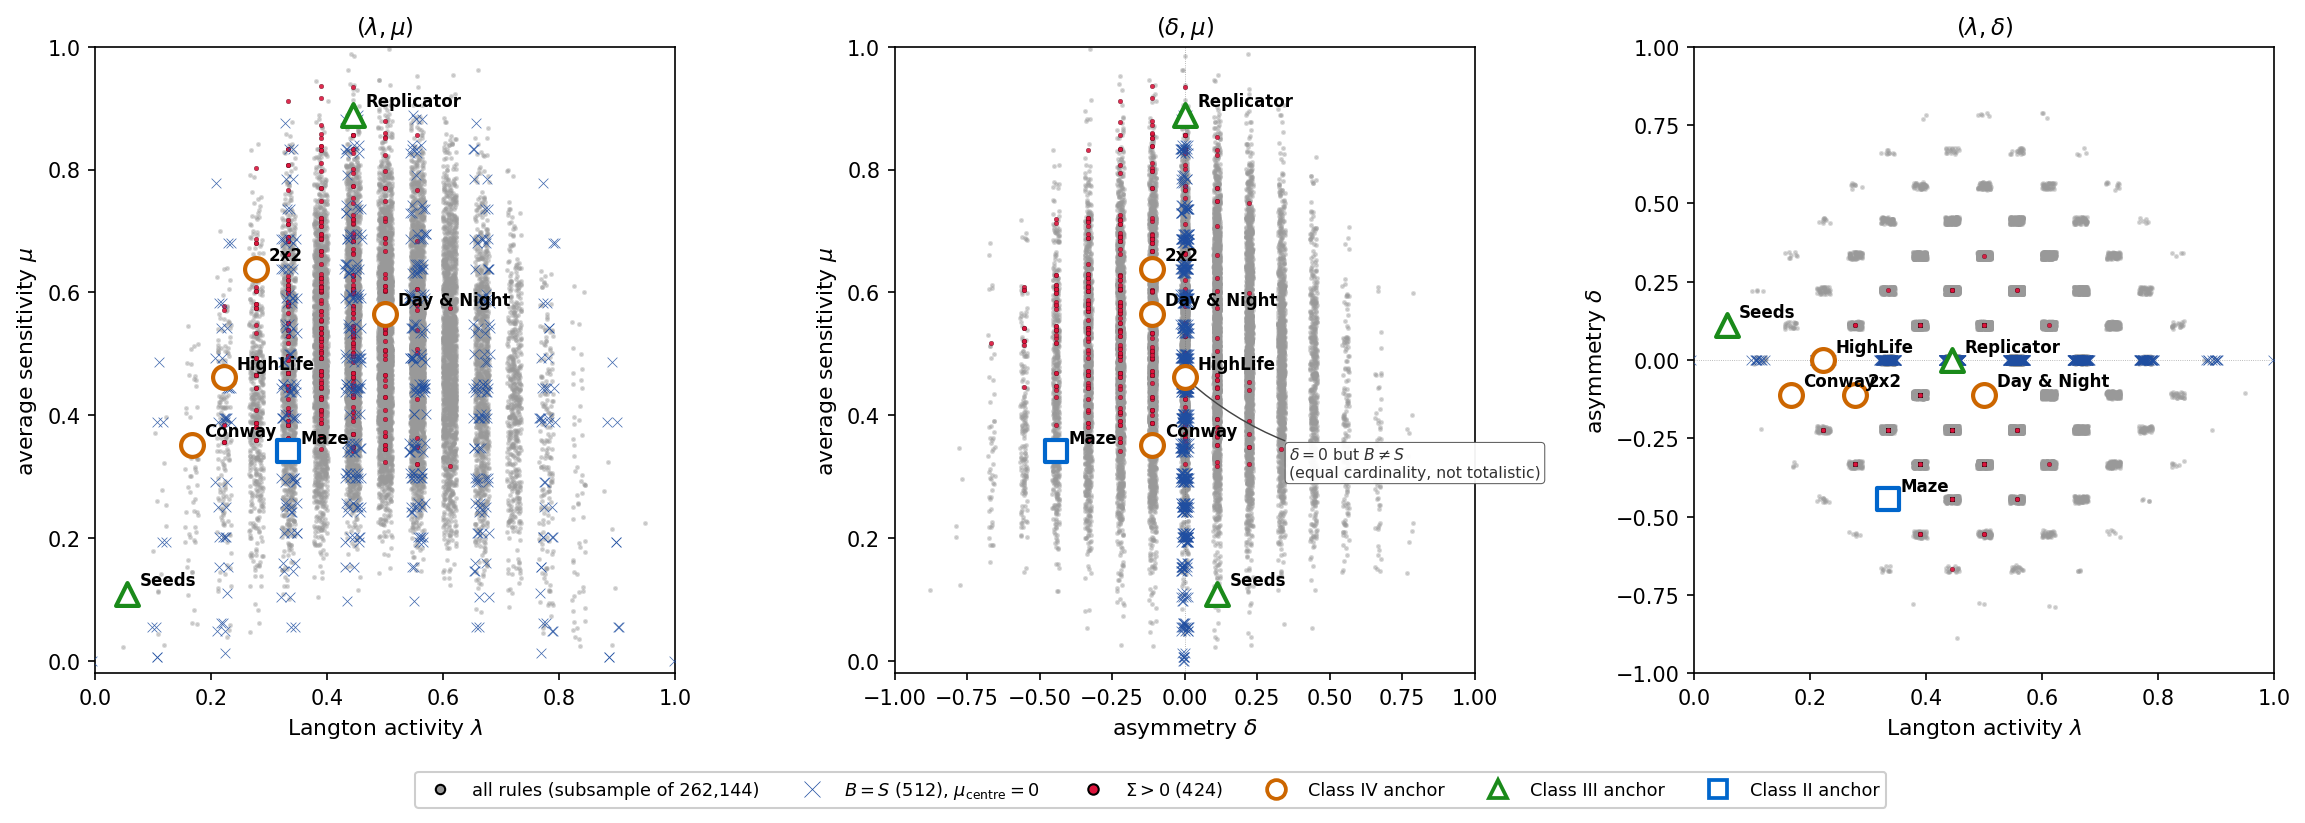
\includegraphics[width=\linewidth]{figures/binder_lambda_mu.png}
% AGENT: confirm filename (3-panel figure).
\caption{Three coordinate projections of all $262{,}144$ rules (grey subsample),
the $512$ fully totalistic $B=S$ rules (royal-blue X, $\mu_{\text{centre}}=0$),
and the $424$ rules with $\Sigma>0$ (crimson). Anchors are outlined markers
coloured by Wolfram class. $(\lambda,\mu)$: $B=S$ rules trace the
$\mu_{\text{centre}}=0$ locus, $\Sigma>0$ rules sit off it. $(\delta,\mu)$: $B=S$
rules collapse to $\delta=0$ while $\Sigma>0$ rules cluster at $\delta\approx-0.2$.
$(\lambda,\delta)$: $\Sigma>0$ rules form a diamond near $(0.4,-0.2)$. HighLife
and Replicator lie on $\delta=0$ by equal cardinality without being totalistic,
illustrating the $\delta=0$ vs.\ $B=S$ distinction of \S\ref{sec:coords}.}
\label{fig:planes}
\end{figure}

\subsection{Combinatorial spaceship support and the $B=S$ exclusion}
\label{sec:results-sigma}

Of the $262{,}144$ rules, $\Sigma>0$ holds for $424$ ($0.16\%$); these cluster in
the $(\lambda,\delta)$ diamond near $(0.4,-0.2)$, overlapping Conway. They support
$876$ distinct orbit-representative spaceships, of which $560$ are diagonal and
$316$ orthogonal, with no $3{\times}3$ knight-ship; the period distribution peaks
at $T=4$. Direction is a clean per-rule property: of the $424$, $300$ support only
diagonal ships and $124$ only orthogonal, none both at the $3{\times}3$ footprint.
Only Conway and HighLife appear among the project's canonical anchors, leaving
many previously uncatalogued rules that support a compact glider---though, as
\S\ref{sec:disc-conway} shows, those with genuinely Conway-like bulk dynamics turn
out to be anchor variants rather than new rules (Figure~\ref{fig:sigma}).

\paragraph{The $B=S$ exclusion and its footprint dependence.}
The $512$ rules with $B=S$ (equivalently $\mu_{\text{centre}}=0$) contain
\emph{zero} rules with $\Sigma>0$ at any $T\le16$, against the bulk rate of
$0.16\%$. This is the sharp form of ``exclude, not certify'': a single
cardinality-blind coordinate, $\mu_{\text{centre}}$, rules out compact
propagation outright on its zero set. The exclusion is specific to the compact
footprint. Enumerating larger seeds exhaustively over all $B=S$ rules, $36$ of
the $256$ vacuum-stable ones support a $4{\times}4$ spaceship and $40$ a
$5{\times}5$ one (against $0$ at $3{\times}3$), so $\mu_{\text{centre}}=0$ closes
the \emph{compact} propagation channel, not propagation at all scales. The
recovery is bounded, not monotone toward parity: the count saturates near $15\%$
of vacuum-stable $B=S$ rules, and \emph{build-and-hold}---a glider together with
static storage---remains rare, holding for $4$ rules at $4{\times}4$ and $8$ at
$5{\times}5$ (counting still lifes; every glider-bearing rule oscillates, so
oscillation is not an informative storage test here). Moreover the gap to Conway
\emph{widens} with footprint: the still-life count of the richest such $B=S$ rule
trails Conway's by $6.3\times$ at $4{\times}4$ and $9.2\times$ at $5{\times}5$. A
rule forced onto the diagonal tunes propagation and storage with a single set and
cannot exploit a larger window on both axes at once, as a rule with independent
$B$ and $S$ can; the strict $3{\times}3$ exclusion therefore softens into a
widening handicap rather than vanishing. The combinatorial recovery does not,
however, bring behavioural complexity with it. Running the richest build-and-hold
candidates---the rules that combine a larger-footprint glider with the most still
lifes---from random initial conditions across a range of densities, and inspecting
the trajectories directly, we find chaotic (Class~III-like) bulk dynamics: the
field boils to a disordered steady state without the enumerated glider visibly
emerging or persistent objects surviving. Within the footprints examined
($\le5{\times}5$) and the random-initial-condition sampling used, no fully
totalistic rule displays Game-of-Life--like (Class~IV) behaviour; the diagonal
gains combinatorial glider capability at larger scales but not expressed
complexity. We give the mechanism in
\S\ref{sec:disc-mechanism}. (The $4{\times}4$ enumeration is exhaustive over all
$262{,}144$ rules---$8{,}206$ support a spaceship, and the $424$ compact-glider
rules are contained in this set exactly; the $5{\times}5$ enumeration is
exhaustive over $B=S$ but sampled elsewhere.)

\begin{figure}[t]
\centering
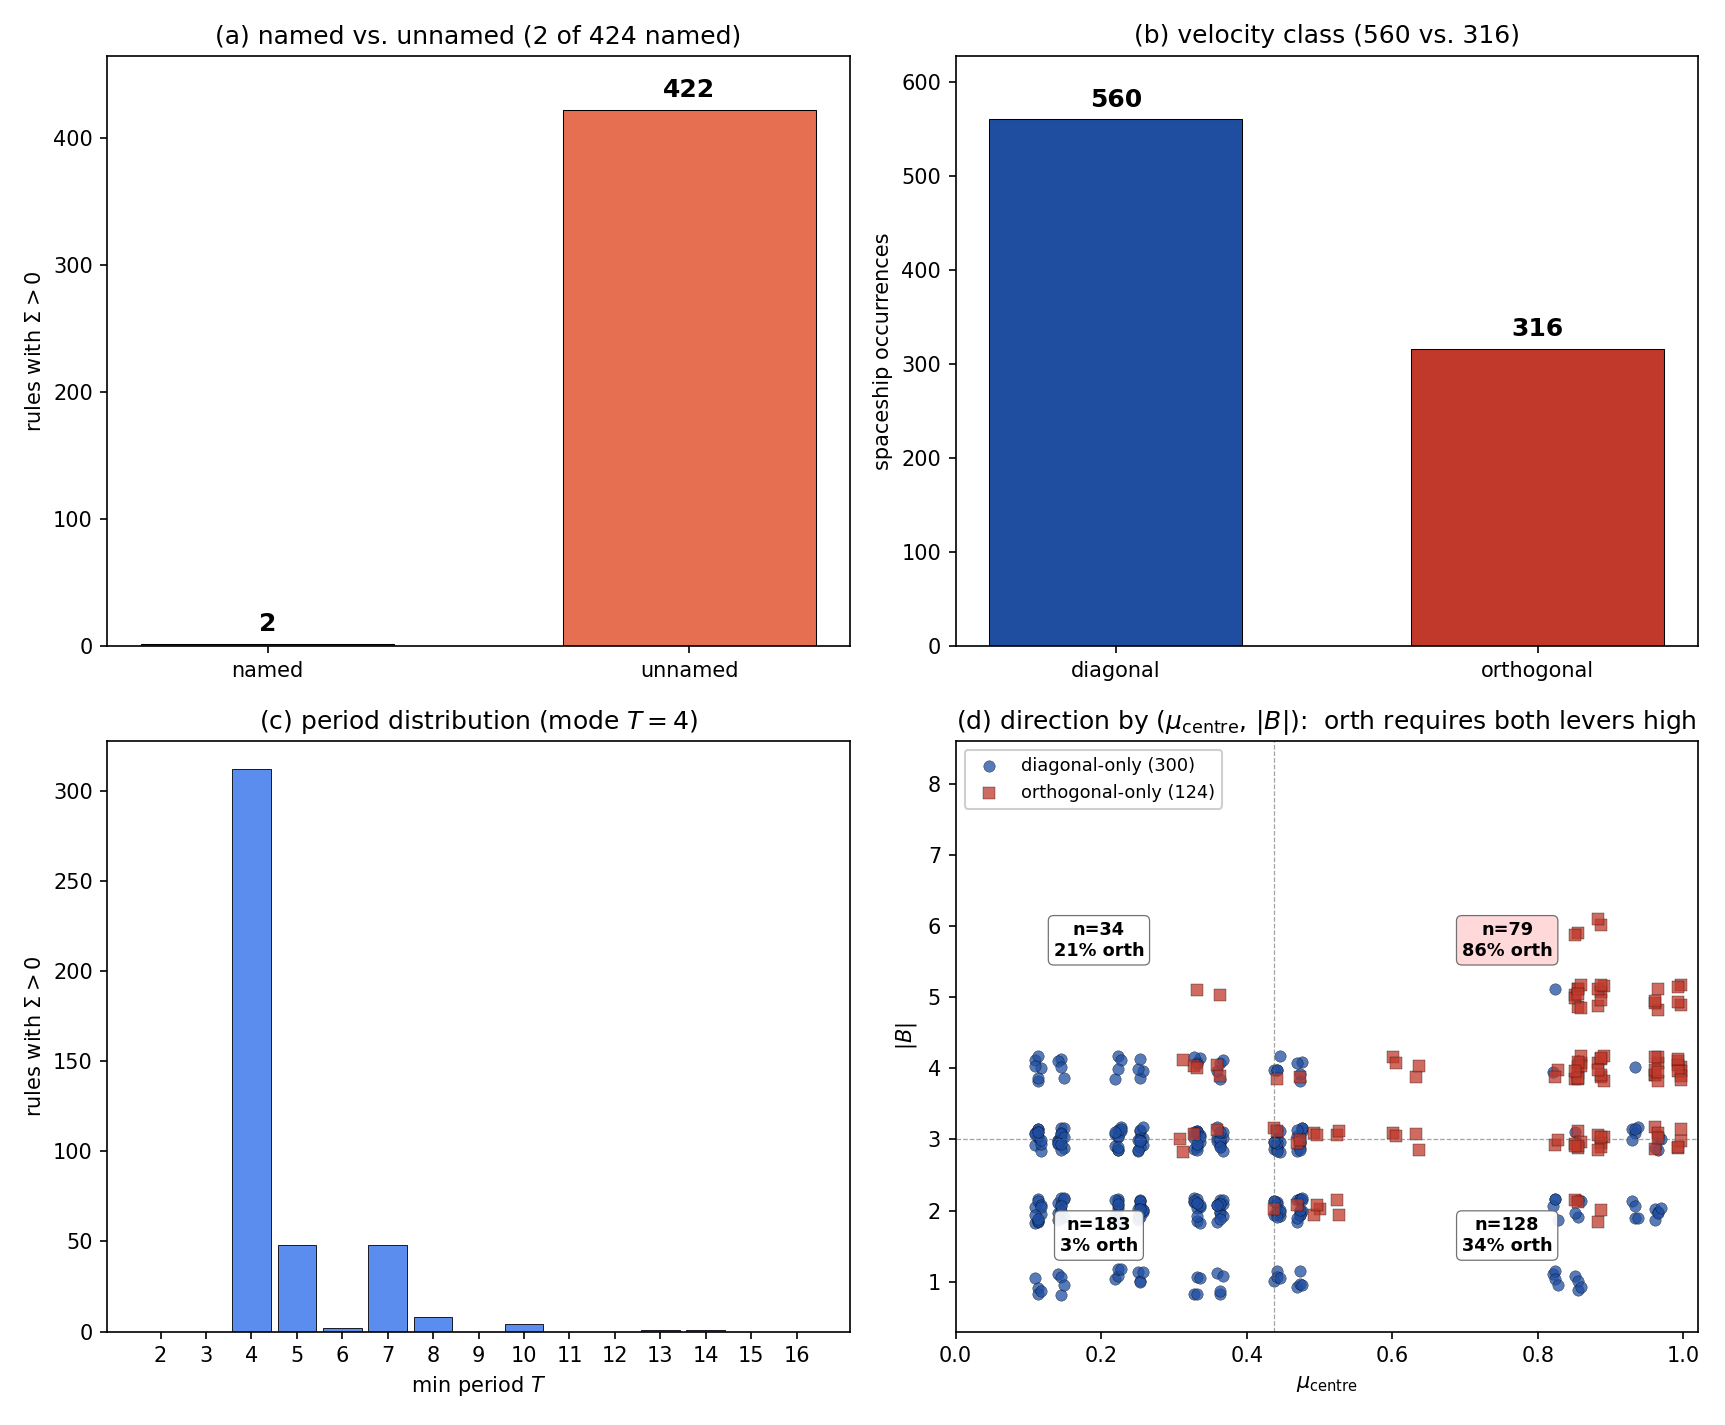
\includegraphics[width=\linewidth]{figures/sigma_characterization.png}
% AGENT: confirm filename (revised 4-panel figure).
\caption{Combinatorial characterisation of the $424$ rules with $\Sigma>0$.
(a)~Named vs.\ unnamed in the canonical anchor list ($2$ of $424$). (b)~Velocity
class at the per-ship level ($560$ diagonal vs.\ $316$ orthogonal). (c)~Period
distribution, mode $T=4$. (d)~Direction in the $(\mu_{\text{centre}},|B|)$ plane:
orthogonal motion requires high $\mu_{\text{centre}}$ \emph{and} large $|B|$
jointly (the joint corner is $86\%$ orthogonal, either lever alone only
$21$--$34\%$, the unfavoured corner $3\%$); diagonal is the default elsewhere
(\S\ref{sec:disc-mechanism}).}
\label{fig:sigma}
\end{figure}

\subsection{Glider-capable but dynamically silent rules}
\label{sec:results-silent}

Cross-referencing $\Sigma$ against $\mathcal{G}^{*}_{\text{alt}}$ isolates a sharp
population that makes the capability/expression gap concrete. We find $33$ rules
that combinatorially support a $3{\times}3$ glider yet produce no coherent
propagation from random initial conditions across a deliberately wide search---$13$
densities $\rho_0\in[0.05,0.90]$, $25$ seeds each, runs of $10^{3}$ steps ($325$
trials per rule). The asymmetry between the two claims is the point. That the
glider \emph{exists} is a construction, not a sample: enumerated from the table and
verified by injecting it onto a quiescent grid, where it propagates steadily. That
random dynamics \emph{do not} produce it is, by contrast, only ever an estimate
over sampled initial conditions; we state it as a measure, not an absolute---the
glider's basin is negligible under random sampling, undetected in those $325$
trials. Capability is certifiable from the table; expression is only estimable
from dynamics. (A further five rules silent at $\rho_0=0.30$ express intermittently
at other densities; they are rare-basin, not silent, and are excluded from the
$33$.)

The obstruction is not a missing background. Every $\Sigma>0$ rule has a stable
dead vacuum by construction---a glider is enumerated on a quiescent background, so
a rule whose vacuum ignited could not register $\Sigma>0$---and indeed all $33$
have $0\notin B$. The glider genuinely lives on empty space; the random-IC
trajectory simply never assembles it there. Measuring the trajectories shows two
opposite failures: $22$ of the $33$ \emph{freeze} (the field settles to
near-vacuum, observed tail densities $\bar\rho\approx0.005$--$0.012$) and $11$
\emph{flood} (the field saturates, $\bar\rho\approx0.58$--$0.99$), with none in
the moderate band $[0.10,0.56]$ that expressing rules---Conway among them---occupy.
On the silent population the split is read by a single survival bit: every flood
rule has $8\in S$ (saturated regions persist; $11/11$), while the freeze rules
have restrictive survival ($\overline{|S|}=4.5$, two-thirds with loneliness death
$0,1\notin S$). This is descriptive of the $33$, not a general law: on a uniform
$3{,}000$-rule sample from the full $262{,}144$, ranking rules by activity
$\lambda$ alone recovers the flood-versus-freeze (dense-versus-sparse
settling) split in the large majority of pairwise comparisons---about
$86\%$---while no simple birth/survival set relation predicts the split
out of sample. The silent rules are those
whose glider-bearing birth set pairs with a survival rule that drives the
trajectory out of the viable band, too dense or too sparse for the glider to
persist on clean background. Which regime a rule falls into is determined by the
table but not reducible to a closed-form predictor of it: a mean-field density map
reproduces the gross density ordering across rules (rank correlation $0.77$ with
measured $\bar\rho$, against $0.34$ for the best single-bit feature) yet
mis-places most silent rules at a moderate interior fixed point
($\rho\approx0.4$) the spatially-fragmenting dynamics never reach. The regime must
be simulated---the dynamical counterpart of ``certifiable versus estimable.''

A controlled witness fixes capability and isolates the survival rule. The family
$B=\{3\}$ contains rules that share a common supported diagonal glider, Conway
among them. Holding the glider fixed and varying only $S$, some express it from
random ICs and others do not: Conway's $S=\{2,3\}$ does, while
$B\{3\}/S\{2,4,5,8\}$---the same birth set, the same supported glider---does not.
Expression is thus not a function of capability alone. Propagation capacity is set
by $B$; whether random dynamics express it depends on $S$ (\S\ref{sec:disc-conway}).

\subsection{Hierarchical $B/S$ factorisation of propagation and storage}
\label{sec:results-factor}

Define the propagation-enabling birth sets $\mathcal{B}_{\text{prop}}=\{B:|\{S:
\Sigma(B,S)>0\}|\ge4\}$. Only $24$ of $512$ birth sets ($4.7\%$) qualify,
dominated by $B\supseteq\{3\}$ variants; outside $\mathcal{B}_{\text{prop}}$
propagation capacity is essentially absent. Within the enabled slice ($12{,}288$
rules) the Spearman correlation between still-life count and $|S|$ is $0.555$;
outside the slice it drops to $0.135$ (Figure~\ref{fig:factor}). The factorisation
is hierarchical, not symmetric: $B$ gates whether any structure is possible, $S$
tunes storage richness once the gate is open.

\paragraph{In-place recurrence forms one storage axis.}
Enumerating in-place oscillators by the same protocol, $57{,}270$ rules
($21.85\%$) have $\Omega>0$; all $424$ $\Sigma>0$ rules are among them, $56{,}846$
oscillate without any spaceship, and none support a spaceship without also
oscillating. Oscillation is birth-gated through a strictly wider gate:
$|\mathcal{B}_{\text{osc}}|=128$ against $|\mathcal{B}_{\text{prop}}|=24$,
and storage (any still life) through a wider one still,
$|\mathcal{B}_{\text{sl}}|=176$; the three form a strict three-level
nesting $\mathcal{B}_{\text{prop}}\subset\mathcal{B}_{\text{osc}}
\subset\mathcal{B}_{\text{sl}}$
($24\subset128\subset176$ of $512$; Figure~\ref{fig:factor}a).
Storage is thus wider than oscillation---modestly, not vastly---and
propagation is the narrowest gate. We find
Spearman $\rho(\Omega,\#\mathrm{SL})=+0.825$ against $\rho(\Omega,\Sigma)=+0.080$;
the informative quantity is the contrast, not the magnitude (still lifes and
oscillators are the same enumeration at period $1$ and $\ge2$, so a strong
correlation is expected). The relevant partition is not static-versus-moving but
translating-versus-non-translating: in-place recurrence at any period forms a
single $S$-tuned storage axis, and translation is orthogonal to it for a
structural reason---it needs the centre-bit asymmetry $\mu_{\text{centre}}>0$ that
the in-place objects do not. The $B=S$ submanifold confirms this directly: $B=S$
rules support oscillators at $96/512=18.75\%$ (within reach of the $21.85\%$
full-space rate, all at period $T=2$) while supporting $0/512$ compact spaceships.
$\mu_{\text{centre}}=0$ closes the translation channel specifically and leaves the
in-place storage channel essentially intact (Figure~\ref{fig:factor}; mechanism in
\S\ref{sec:disc-mechanism}).

\paragraph{$\delta$ as the factorisation axis, $\delta_{\text{edge}}$ as a secondary one.}
Because the factorisation is intrinsically a birth-versus-survival statement, the
$\tau$-odd coordinate $\delta$ is its natural projection. Among the $424$
$\Sigma>0$ rules the $\delta$ distribution is sharply skewed to $\delta<0$ (median
$-0.222$, $340$ of $424$ below zero), whereas the $\Sigma=0$ bulk is symmetric
about zero by the $\tau$-symmetry of rule space (Figure~\ref{fig:tauodd}). This
$\delta\approx-0.22$ is, for the asymmetry axis, the analogue of Langton's
critical $\lambda\approx0.25$ for the activity axis: a single scalar value where
capability concentrates. But the paper's framing applies to it in full---both
$\lambda$ and $\delta$ \emph{locate} without \emph{certifying}. The same
$\delta\approx-0.22$ slice is shared by thousands of $\Sigma=0$ rules, so landing
on it is necessary for the propagation--storage structure but never sufficient for
a glider; the value marks a region, not a guarantee. This fingerprint is specific
to the compact footprint: among the $8{,}206$ rules that support a $4{\times}4$
spaceship the $\delta$ skew washes out (median $0$, rank-biserial $-0.12$ against
$\approx-0.5$ at $3{\times}3$), because a wider window admits birth-heavier
orthogonal shippers. What survives footprint widening is the \emph{gate}
structure, not the $\delta$ sign: the $24$ birth sets of
$\mathcal{B}_{\text{prop}}^{3\times3}$ are contained in the $64$ of
$\mathcal{B}_{\text{prop}}^{4\times4}$ exactly, and both remain dominated by small
birth sets (mean $|B|=3.5$ at $4{\times}4$, against a uniform peak at $|B|=5$). The
birth-light asymmetry is thus what \emph{compact} propagation costs, not a
universal law; the narrow gate of small birth sets is the footprint-robust core.
The
$\tau$-odd, $\sigma$-odd coordinate $\delta_{\text{edge}}$, orthogonal to
$(\lambda,\delta,\mu)$ on the full space, carries a genuine but secondary signal:
$\Sigma>0$ rules favour a birth set that is both small ($\delta<0$) and contiguous
($\delta_{\text{edge}}<0$). Because we enumerate the entire rule population rather
than a sample, we read these as effect sizes, not significance: conditional on
$(\lambda,\delta,\mu)$ the $\delta_{\text{edge}}$ logistic coefficient retains
about one quarter the magnitude of $\delta$'s ($\beta=-0.21$ vs.\ $-0.78$), and
stratifying by $\delta$ leaves about
$70\%$ of the marginal shift---a contiguity preference on top of small cardinality,
not a co-equal second axis. The four parity sectors
$(\lambda,\delta,\mu,\delta_{\text{edge}})$ together form a complete
Boolean-derivative parametrisation; the $(\text{odd},\text{odd})$ sector is
mechanism-consistent but quantitatively subordinate to $\delta$.

\begin{figure}[t]
\centering
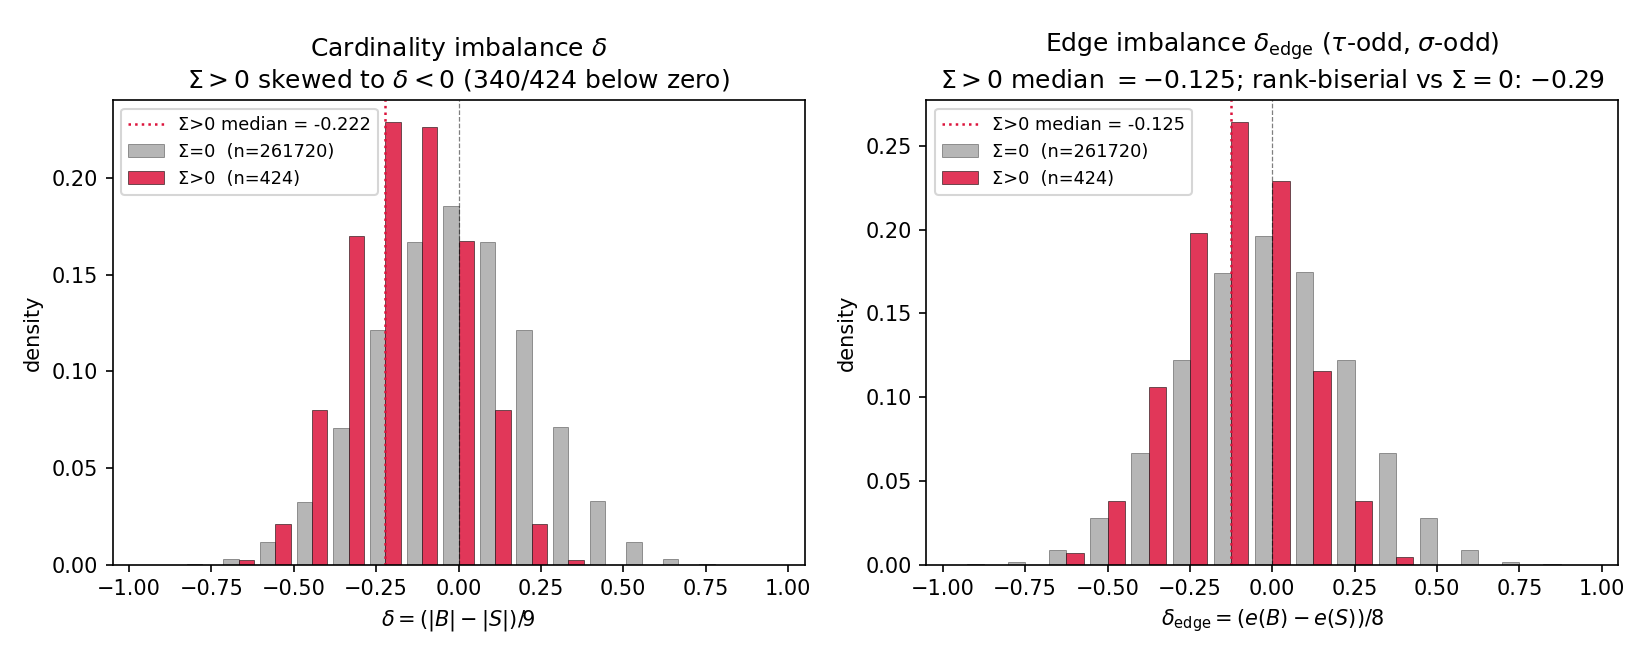
\includegraphics[width=\linewidth]{figures/Fig_delta_histograms.png}
% AGENT: confirm filename.
\caption{Histograms of the two $\tau$-odd coordinates over all $262{,}144$ rules.
Grey: $\Sigma=0$ bulk; crimson: $\Sigma>0$ ($n=424$). Left: $\delta$, symmetric
about zero on the bulk (forced by $\tau$-symmetry) but sharply skewed to
$\delta<0$ for $\Sigma>0$ (median $-0.222$). Right: $\delta_{\text{edge}}$, a
similar but partly inherited marginal shift (median $-0.125$); conditional on
$(\lambda,\delta,\mu)$ it retains about a quarter of $\delta$'s magnitude.}
\label{fig:tauodd}
\end{figure}

\begin{figure}[t]
\centering
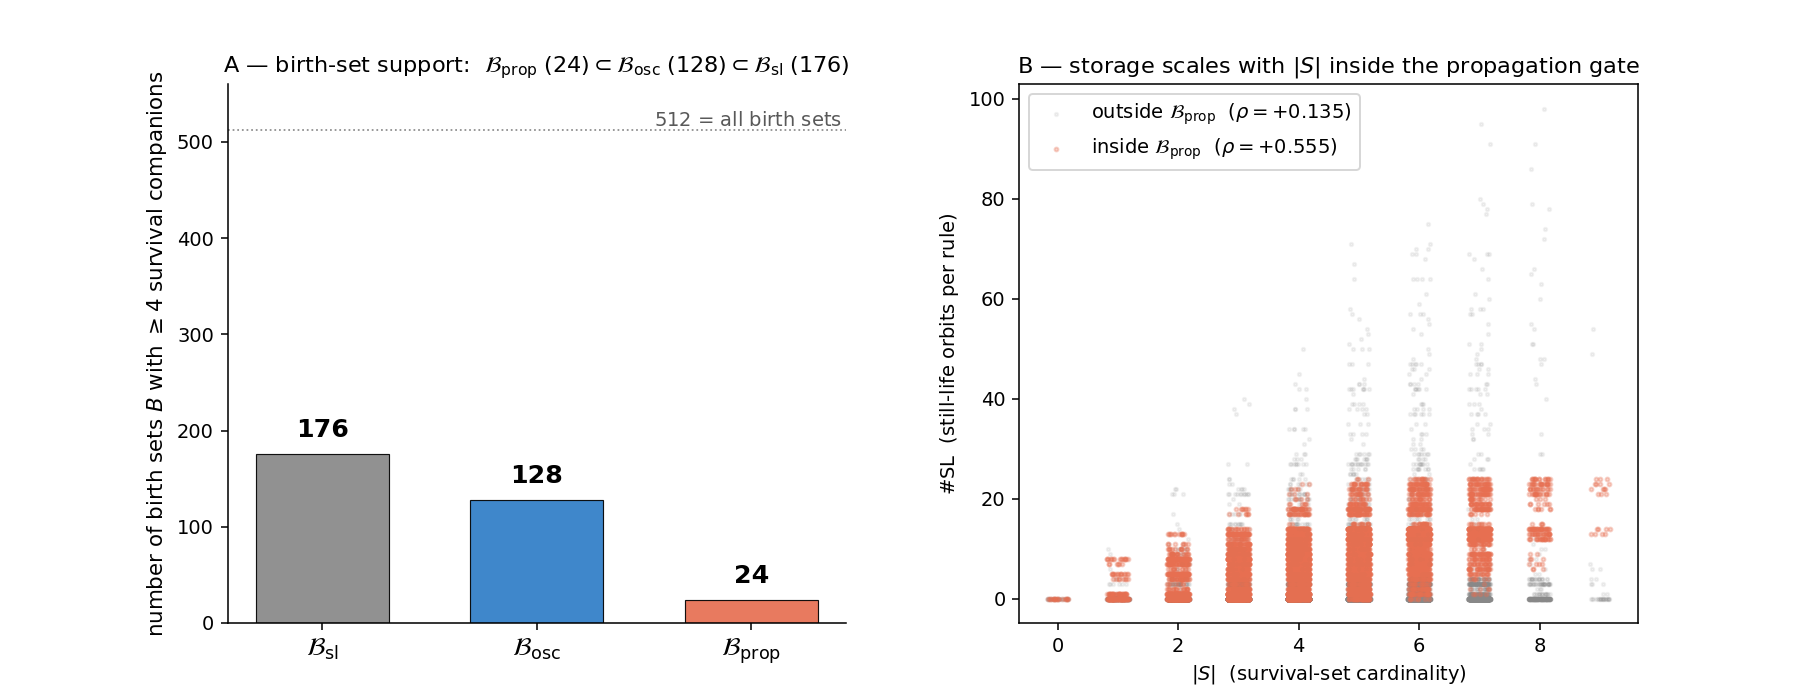
\includegraphics[width=0.92\linewidth]{figures/factorization.png}
% AGENT: confirm filename.
\caption{Hierarchical $B/S$ factorisation.
(a)~Birth-set support of each capability at threshold $k\ge4$ companions
(a birth set counts as supporting a structure iff at least $4$ of the $512$
possible survival companions $S$ yield it): $|\mathcal{B}_{\text{sl}}|=176$
(still lifes) $\supset|\mathcal{B}_{\text{osc}}|=128$
(oscillators) $\supset|\mathcal{B}_{\text{prop}}|=24$ (spaceships),
nested strictly within the $512$ birth sets---propagation is the narrowest
gate, oscillation wider, storage widest. At the looser $k\ge1$ threshold
$|\mathcal{B}_{\text{prop}}|=26$ (two borderline birth sets with only two
companions each drop out at $k\ge4$); the storage and oscillation counts
are unchanged. (b)~$\#\mathrm{SL}$ against survival-set cardinality $|S|$,
split by $B\in\mathcal{B}_{\text{prop}}$ (orange) vs.\ outside (grey):
inside the propagation gate storage tunes with $|S|$
(Spearman $\rho=0.555$), outside it does not ($\rho=0.135$).}
\label{fig:factor}
\end{figure}

\begin{figure}[t]
\centering
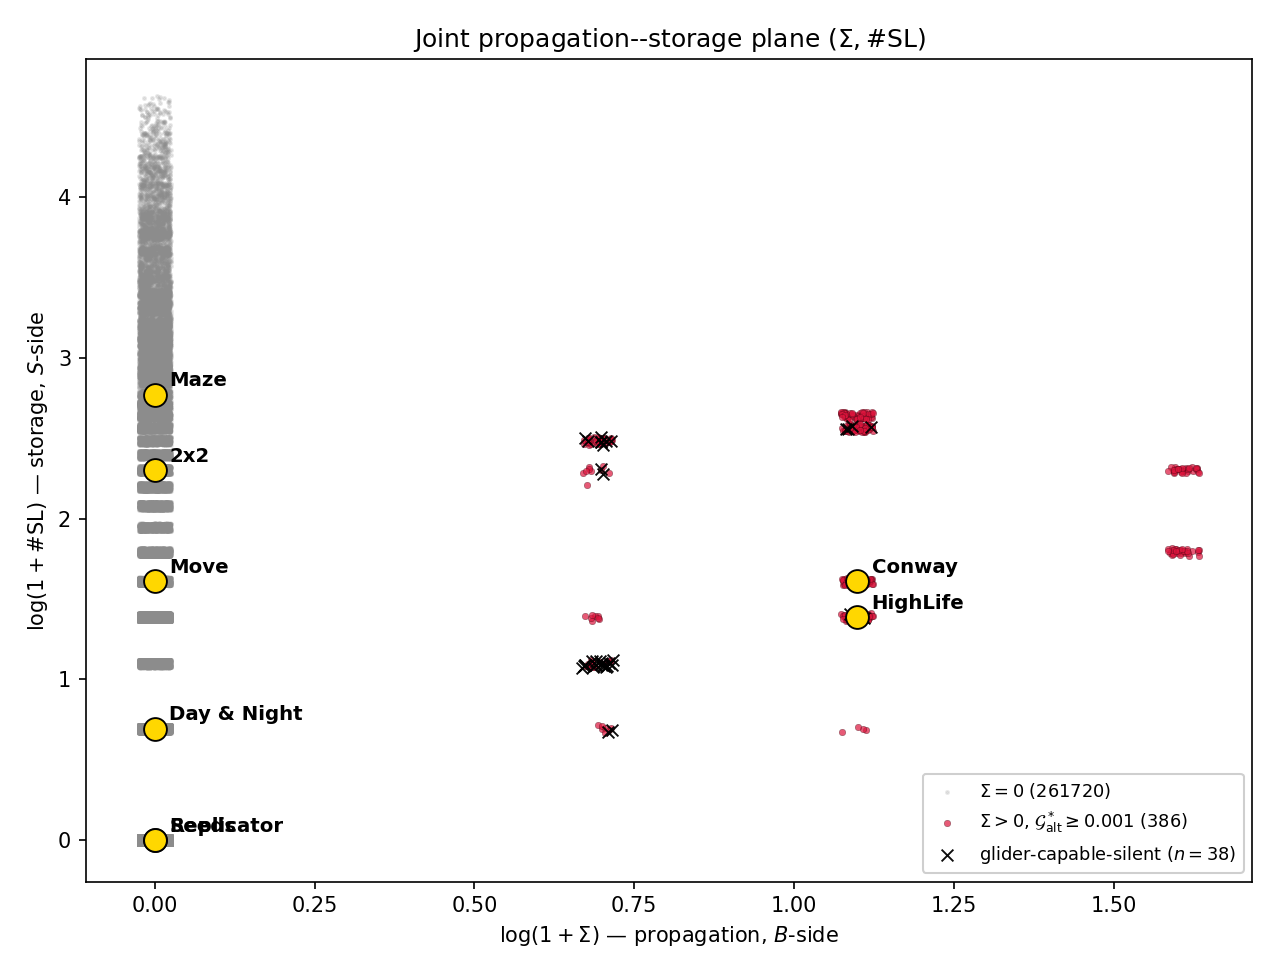
\includegraphics[width=0.7\linewidth]{figures/joint_plane.png}
% AGENT: confirm filename.
\caption{Joint propagation--storage plane $(\Sigma,\#\mathrm{SL})$ in $\log(1+x)$
coordinates. Conway and HighLife sit in the upper-right corner (both gliders and
rich storage). The $\Sigma=0$ column supports no \emph{compact} glider and
contains the Class~IV anchors $2{\times}2$, Day~\&~Night and Move---whose
complexity rests on engineered, large-footprint propagation this enumeration does
not capture (\S\ref{sec:disc-conway})---while Seeds and Replicator sit at the
origin. The $38$ marked ``glider-capable-silent'' points are the initial
silent population from the main sweep, subsequently resolved as $33$
robustly silent and $5$ rare-basin rules (\S\ref{sec:results-silent}); this
$38$ is distinct from the $38$-rule pre-floor count of the census screen in
\S\ref{sec:disc-conway}, which the two sets happen to share by coincidence.}
\label{fig:joint}
\end{figure}

\subsection{Capability is a rule-table property, not a dynamical one}
\label{sec:results-gap}

The silent population shows by example that combinatorial capability need not be
expressed by random dynamics. We confirm this with the intrinsic-versus-realised
sensitivity gap $\mathrm{gap}(f)=\mu(f)-\langle\mathrm{sens}\rangle$, where
$\langle\mathrm{sens}\rangle$ averages the Boolean sensitivity over visited rather
than uniform configurations. The gap separates the Wolfram-class regimes cleanly
(positive for the propagating Class~IV anchors Conway and HighLife, negative for
the Class~III chaos anchors Seeds and Replicator). But asked to separate
$\Sigma>0$ from $\Sigma=0$ across the enumerated set, the median gaps differ by
only $-0.34$ vs.\ $-0.36$, indistinguishable against the intra-class spread. The
gap is a clean regime descriptor but not a detector of compact-glider
support---a direct measurement of the obstruction the silent population
illustrates. Capability is certifiable from the table; the dynamical observables
of the sweep track regime, not capability, and are reported as such.

\section{Discussion}

\subsection{The mechanism of the $B=S$ exclusion}
\label{sec:disc-mechanism}

A compact spaceship needs a leading edge that creates state ahead (a
$B$-condition) and a trailing edge that clears state behind (an
$\overline{S}$-condition), on overlapping neighbour-count regions.
$\mu_{\text{centre}}=0$ means the rule is indifferent to a cell's own state at
every count, so it cannot resolve the two geometrically-distinct ``ahead'' and
``behind'' events---a dead cell becoming live and a live cell dying for the same
neighbour configuration---into different outputs. This becomes decisive at the
compact footprint for a geometric reason. A $3{\times}3$ pattern is exactly the
Moore neighbourhood of a single cell: every cell of the object lies within the
neighbourhood of every other, so the object fits entirely inside the field of
view of one cell in one update. Its leading and trailing edges are therefore
never independently addressable---no cell can respond to one without seeing the
other---so a rule that cannot distinguish a cell's own state
($\mu_{\text{centre}}=0$) is forced to treat the ``create ahead'' and ``clear
behind'' events identically, and the compact channel closes. A $4{\times}4$ or
larger object breaks this containment: its extremal cells fall outside one
another's neighbourhoods, so leading and trailing edges can be driven by
disjoint local configurations that $\mu_{\text{centre}}=0$ no longer collapses.
This is precisely why the exclusion is exact at $3{\times}3$ and softens as the
footprint grows---the single-neighbourhood confinement that makes ``compact''
meaningful is exactly the condition under which centre-blindness is fatal.
The exclusion itself is an exhaustive combinatorial fact (no $B=S$ rule registers
a compact spaceship); the centre-cell account here is our explanation of why,
tied to a single coordinate. The oscillator results
localise it exactly: $\mu_{\text{centre}}=0$ closes the \emph{translation} channel
specifically, because translation needs the leading/trailing asymmetry while
in-place recurrence does not; $B=S$ rules oscillate at near-background rate and
are excluded only from compact spaceships. This mechanism is heuristic, not yet a
theorem (\S\ref{sec:disc-limits}): the exclusion is proven by enumeration, but a
proof \emph{from} the centre-cell argument remains open.

The same centre-bit coordinate also grades the \emph{direction} of translation
at the compact footprint (Figure~\ref{fig:sigma}d): among $3{\times}3$ spaceships
orthogonal motion is confined to rules simultaneously high in $\mu_{\text{centre}}$
and large in $|B|$ (the joint corner is $86\%$ orthogonal, either lever alone only
$21$--$34\%$), with diagonal the default elsewhere. The two coordinates act roughly
additively and neither is reducible to the other. This diagonal dominance is
itself compact-specific and inverts with footprint: at $4{\times}4$ orthogonal
spaceships outnumber diagonal ones by roughly seven to one, the reverse of the
$3{\times}3$ ratio. The geometric reading---that axial motion needs a sharper,
denser leading edge than diagonal motion, and that the extra row of a wider window
supplies exactly the structure orthogonal motion requires---we offer only as a
hypothesis.

For storage the binding constraint is a $B$-condition---a still life persists only
if its surrounding dead cells have counts outside $B$---while which interior
configurations survive is set by $S$. This is why $\#\mathrm{SL}$ correlates with
$|S|$ only once one conditions on $B\in\mathcal{B}_{\text{prop}}$, closing the
factorisation: $B$ gates, $S$ tunes.

\subsection{Conway's specialness}
\label{sec:disc-conway}
Conway sits at the intersection of three conditions, the first two combinatorial
and the third dynamical: $B=\{3\}\in\mathcal{B}_{\text{prop}}$ admits the glider;
$S=\{2,3\}$ supports rich still lifes; and the random-IC attractor at
$\rho_0=0.30$ routes trajectories into a regime that visits the glider on clean
background. Rules in the $B=\{3\}$ family share a common supported glider---the
first two conditions hold for every one of them---but only a survival rule that
keeps the trajectory in the moderate-density band, neither flooding nor freezing,
lets random dynamics express it. Conway's $S$ is privileged not because it enables
the glider but because it places the dynamics where the glider can appear.

We can ask the converse question directly: among the rules that support both a
glider and a still life but are absent from the standard catalogue, are any
\emph{dynamically} Conway-like---not merely capable, but producing a
Game-of-Life--style ecology of blinkers, blocks and other small objects from
random starts? Of the $424$ rules with $\Sigma>0$, the $2$ named anchors and $2$
further rules with no still life ($\#\mathrm{SL}=0$) are set aside, leaving $420$
uncatalogued build-and-hold rules. We screen these on \emph{behavioural} criteria
alone---a stabilising tail density (met by $314$ of the $420$ at some density),
followed by a direct census requiring that canonical Game-of-Life still lifes and
oscillators dominate the small live structures, plus a richness floor of at
least one canonical still life (block, beehive, loaf, boat or tub) present in
the tail, so that a rule producing only sparse blinkers---which are canonical
oscillators and would trivially satisfy the raw dominance test---does not
qualify. All criteria are applied \emph{without}
reference to the rule table, so that table similarity is a finding rather than a
filter. Without the richness floor $38$ rules pass; with it, $24$
remain, and the $14$ excluded are precisely the blinker-only degenerates whose
census is Life-like in the letter but not in the spirit. Only then do we compare
the $24$ rich-ecology rules' tables to the anchors: \emph{all $24$} agree with
Conway or HighLife on every visited
$(\text{centre},\text{count})$ pair ($15$ Conway, $9$ HighLife), differing only at
neighbour counts $7$ and $8$, which require locally saturated regions and do not
fire at the tested density. So every uncatalogued
rule that both stabilises and grows a rich Life-like object ecology from random
starts is, on its visited configurations, a Conway or HighLife variant---the
pool contains no rule whose table is distinct from both anchors yet reproduces
their small-object zoo. This is the converse of the paper's
leading theme---capability resides in the table but need not be
expressed---made concrete on the expression side: two rules can differ wherever
their tables are defined yet be dynamically indistinguishable, because behaviour
is fixed by the table only on the configurations a trajectory visits. We stress
the scope: the screen identifies rules Game-of-Life--\emph{like} in their small-object
ecology, not the complete set of dynamically interesting rules---a rule with a rich
but non-Life-like object zoo would pass unrecognised---and the anchor identity is
scoped to the tested densities, where the differing high count is rare rather than
combinatorially impossible.

Both results are, at root, a genotype--phenotype distinction. The rule table is
the genotype: it fixes what is possible and can be read directly, which is why
capability is \emph{certifiable}. What a random trajectory develops is the
phenotype: it depends on initial conditions and dynamics, so it can only be
\emph{estimated}, and it need not realise everything the genotype permits---a rule
may carry a glider it never expresses (\S\ref{sec:results-silent}), just as two
distinct genotypes may yield the same phenotype when the differing genes are never
transcribed (the anchor variants above). The birth--survival asymmetry $\delta$
adds a smaller morphological note: translation requires a rule that distinguishes
``ahead'' from ``behind'', a broken front--back symmetry that in-place recurrence
does not need---loosely, the asymmetry that a moving body plan requires and a
radially symmetric one does not.

\paragraph{External corroboration, and the scope of the claim.}
Comparing against the literature's catalogue of complex life-like rules sharpens
both what these results establish and what they do not. Of twenty rules recorded
as Class~IV or computationally universal in the standard
references~\cite{eppstein2010,adamatzky2010}, exactly one is totalistic
(Replicator), and it is Class~III rather than Class~IV: \emph{every} known
Class~IV rule in the family is non-totalistic. The $B=S$ exclusion is therefore
corroborated externally, not only by our enumeration. Second, our behavioural
screen, run without reference to the literature list, independently recovered four
of these named rules---DryLife, EightLife, Pedestrian~Life and LowDeath---and the
subsequent table comparison correctly identified each as a Conway- or
HighLife-family rule differing only at unvisited high neighbour counts. Third, and
against these, the scoping must be stated plainly. Eleven of the twenty have
$\Sigma_{3\times3}=0$ and so could never enter our screen: Day~\&~Night
($\lambda=0.500$, $\mu=0.565$), $2{\times}2$, Move and Life~without~Death are
complex through \emph{engineered} constructions and large-footprint propagation
that a compact $3{\times}3$ enumeration cannot see. A vanishing compact-glider
count therefore does not imply dynamical simplicity, and the $\Sigma=0$ column of
Figure~\ref{fig:joint} mixes inert rules with rules whose propagation is merely
non-compact. The six \emph{spontaneous} Class~IV rules---the Conway family---do
cluster where our coordinates predict ($\lambda\in[0.17,0.22]$,
$\mu\in[0.35,0.46]$, $\delta\le0$). Our claim is accordingly the narrow one: among
rules supporting a compact glider, spontaneous Game-of-Life--like ecology
concentrates on Conway, HighLife and their behaviourally redundant variants. It is
not the claim that these are the family's only complex rules---they demonstrably
are not.

\subsection{Limitations and open directions}
\label{sec:disc-limits}

The main enumeration is at $3{\times}3$ footprint, $T\le16$, exhaustive over all
$262{,}144$ rules. The $4{\times}4$ enumeration is also exhaustive over all rules
($8{,}206$ support a spaceship, $3.13\%$); the $5{\times}5$ enumeration is
exhaustive over the $512$ $B=S$ rules and sampled elsewhere. Three footprint
observations follow. First, containment is perfect---all $424$
$\Sigma_{3\times3}>0$ rules retain $\Sigma_{4\times4}>0$, with $7{,}782$ further
rules gliding only at $4{\times}4$---so the compact enumeration is a strict lower
bound on propagation capability. Second, the storage axis is scale-invariant
(within-slice Spearman $\rho(\#\mathrm{SL}, |S|) = 0.544$ at $3{\times}3$ and
$0.556$ at $4{\times}4$). Third, the $B=S$ exclusion is compact-specific but does
not simply dissolve with scale: $36$ of the $256$ vacuum-stable $B=S$ rules admit
a $4{\times}4$ spaceship and $40$ a $5{\times}5$, yet those that combine a glider
with static storage stay rare ($4$, then $8$) and fall progressively further from
Conway (still-life gap $6.3\times$ at $4{\times}4$, $9.2\times$ at $5{\times}5$),
so the strict exclusion softens into a widening handicap. $6{\times}6$ and beyond
are presently out of reach in both time and memory (the number of $D_4$
orbit-representative $n{\times}n$ seeds grows from $\sim10^2$ at $3{\times}3$ to
$\sim10^4$, $\sim10^6$, and $\sim10^9$ at $4$-, $5$-, $6{\times}6$).
The factorisation and the $\mu_{\text{centre}}$ mechanism are established
empirically and argued heuristically; a proof that no $B=S$ rule admits a compact
spaceship would convert the $3{\times}3$ exclusion into a theorem and is plausible
from the centre-bit argument. The silent population was characterised across a
$13$-density, $25$-seed sweep, but the underlying claim remains a measure, not an
absolute: a basin of vanishing but nonzero weight cannot be excluded by sampling.
A follow-up seeded with known spaceships rather than random ICs would map the
basin structure directly, and the flood/freeze regime that gates
expression---determined by the table yet not captured by a mean-field
predictor---invites a sharper theory of which rules settle into the
moderate-density band that propagation requires.

\appendix
\section{The bit-flip duality and the dynamical sweep}
\label{app:dynamical}

The bit-flip duality $\sigma$ (\S\ref{sec:symm}) is exact at the level of
trajectories ($g(\lnot x)=\lnot f(x)$ for $g=\sigma(f)$) but is broken by sparse
Bernoulli ICs: a rule and its dual visit different attractors from the same IC.
Pairing every sample with its bit-flipped twin (the symmetric-IC ensemble of
\S\ref{sec:dyn}) restores the duality at the level of ensemble means; we verify a
residual twin-gap at the seed-noise floor. The $512$ $\sigma$-fixed points (e.g.\
Day~\&~Night) are the self-dual rules. Beyond $\mathcal{G}^{*}_{\text{alt}}$ the
sweep records per-frame compressibility, a basin-asymmetry index and the cell-flip
rate; gauge-fixed by symmetric-IC averaging these co-locate $\sigma$-twins and
separate canonical anchors into recognisable regimes, but---as
\S\ref{sec:results-gap} shows---do not predict $\Sigma>0$ status and are reported
only as regime descriptors, not capability detectors.

\begin{thebibliography}{Mitchell et al. 1993}
\bibitem[Adamatzky 2010]{adamatzky2010} A.~Adamatzky, editor. \emph{Game of Life Cellular Automata}. Springer, 2010.
\bibitem[Berlekamp et al. 1982]{berlekamp1982} E.~R. Berlekamp, J.~H. Conway, and R.~K. Guy. \emph{Winning Ways for Your Mathematical Plays, Vol.~2}. Academic Press, 1982.
\bibitem[Binder 1993]{binder1993} P.-M. Binder. A phase diagram for elementary cellular automata. \emph{Complex Systems}, 7:241--247, 1993.
\bibitem[Eppstein 2010]{eppstein2010} D.~Eppstein. Growth and decay in life-like cellular automata. In A.~Adamatzky, editor, \emph{Game of Life Cellular Automata}, pages 71--97. Springer, 2010. (arXiv:0911.2890, 2009.)
\bibitem[Gardner 1970]{gardner1970} M.~Gardner. Mathematical games --- the fantastic combinations of John Conway's new solitaire game ``life''. \emph{Scientific American}, 223(4):120--123, 1970.
\bibitem[Langton 1990]{langton1990} C.~G. Langton. Computation at the edge of chaos: phase transitions and emergent computation. \emph{Physica D}, 42(1--3):12--37, 1990.
\bibitem[Mitchell et al. 1993]{mitchell1993} M.~Mitchell, P.~T. Hraber, and J.~P. Crutchfield. Revisiting the edge of chaos: evolving cellular automata to perform computations. \emph{Complex Systems}, 7:89--130, 1993.
\bibitem[Vichniac 1990]{vichniac1990} G.~Y. Vichniac. Boolean derivatives on cellular automata. \emph{Physica D}, 45(1--3):63--74, 1990.
\bibitem[von Neumann 1966]{vonneumann1966} J.~von Neumann. \emph{Theory of Self-Reproducing Automata}. Edited and completed by A.~W. Burks. University of Illinois Press, 1966.
\bibitem[Wolfram 1983]{wolfram1983} S.~Wolfram. Statistical mechanics of cellular automata. \emph{Reviews of Modern Physics}, 55(3):601--644, 1983.
\bibitem[Wolfram 1984]{wolfram1984} S.~Wolfram. Universality and complexity in cellular automata. \emph{Physica D}, 10(1--2):1--35, 1984.
\bibitem[Wuensche 1999]{wuensche1999} A.~Wuensche. Classifying cellular automata automatically. \emph{Complexity}, 4(3):47--66, 1999.
\end{thebibliography}

\end{document}
